%
% Modelo de trabalho acadêmico para disciplinas em português brasileiro e em 
% conformidade com as normas da ABNT. Melhor visualizado em 80 colunas.
%
% Documento principal
% Data: 18 de março de 2016
%
% *****************************************************************************
% *  Centro Federal de Educação Tecnológica de Minas Gerais - CEFET-MG        *
% *                                                                           *
% *                                                                           *
% *  Autor que adaptou : Augusto Morais <aflavio@gmail.com>                   * 
% *  Source: https://github.com/aflavio/cefet-MG-latex                         
% *                                                                           *
% *                                                                           *
% *  Autor: Henrique E. Borges <henrique@lsi.cefetmg.br>                      *
% *  Autor: Denise de Souza <densouza@gmail.com>                              *
% *  Autor: Cristiano Fraga G. Nunes <cfgnunes@gmail.com>                     *
% *  Autor: Lauro César <https://code.google.com/p/abntex2/                   *
% *                                                                           *
% *****************************************************************************



\documentclass[
      %twoside,         % Impressão em frente (anverso) e verso. Oposto a oneside
      oneside,          % Impressão apenas no anverso. Oposto a twoside
      a4paper,          % Tamanho do papel
      english,          % Idioma adicional para hifenização
      brazilian,        % O ultimo idioma será o principal idioma do documento    
]{abntex2-cefetmg} 



% -----------------------------------------------------------------------------
%    Configura as citações bibliográficas conforme a norma ABNT
% -----------------------------------------------------------------------------

\usepackage[brazilian,hyperpageref]{backref}
\usepackage[alf, 
abnt-emphasize=bf, 
bibjustif, 
recuo=0cm,
abnt-doi=expand,        % Expande um endereço com doi: para http://dx.doi.org/
abnt-url-package=url,   % utiliza o pacote url
abnt-refinfo=yes,       % utiliza o estilo bibliográfico abnt-refinfo
abnt-etal-cite=3, 
abnt-etal-list=3,
abnt-thesis-year=final]{abntex2cite}    % Formata as citações conforme ABNT


% -----------------------------------------------------------------------------
%    Pacotes utilizados 
% -----------------------------------------------------------------------------

\usepackage[utf8]{inputenc}     % Usa codificação UTF-8
\usepackage[T1]{fontenc}        % Seleção de código de fonte

% Fonts: Times, LAtin Modern, Palatino, Latin Modern, Helvetica
\usepackage[scaled]{helvet}		  
\usepackage{scalefnt}			      
%\usepackage{times}				      
%\usepackage{lmodern}			      
%\usepackage{palatino}			    
%\usepackage{lmodern}			      

\renewcommand*\familydefault{\sfdefault} 	

% Inserção de caracteres gregos, matematicos, etc
\usepackage{upgreek}			      
\usepackage{latexsym}			      
\usepackage{amsfonts, amssymb, amsmath, dsfont}		


\usepackage{lscape}             % Páginas em modo "paisagem"
\usepackage{indentfirst}        % Indenta o primeiro parágrafo de cada seção.
\usepackage{microtype}          % Melhora a justificação do documento
\usepackage{hyperref}           % Usado para criar “hyperlinks” no PDF
\usepackage{breakurl}           % Permite quebra de linha em URLs longas
\usepackage{graphicx}           % Inclusão de gráficos e figuras
\usepackage{tikz}               % Pacote para desenhos
\usepackage{color, colortbl}    % Controle das cores
\usepackage[bottom]{footmisc}   % Notas de rodapé sempre na mesma posição
\usepackage{bookmark}           % Cria menu de bookmarks
\usepackage{verbatim}           % Apresenta texto tal como escrito no doc.
\usepackage{multirow, array}    % Permite tabelas com múltiplas linhas e colunas
\usepackage{booktabs}           % Réguas horizontais em tabelas
\usepackage{float}              % Tabelas/figuras em ambiente multi-colunas
\usepackage{subeqnarray}        % Permite subnumeracao de equações
\usepackage{listings}        % Permite subnumeracao de equações

\usepackage[pointedenum]{paralist}              % Listas numeradas/bullets
\usepackage[algoruled, portuguese]{algorithm2e} % algoritmos em Português

\usepackage{makeidx}            % Usado para produzir índice remissivo (glossário)
	\makeindex                  % Compila o índice
	
	
% -----------------------------------------------------------------------------	
%   Pacotes DESABILITADOS POR DEFAULT
% -----------------------------------------------------------------------------
%\usepackage[hyphens]{url}  % Melhora apresentação de URLs
%\usepackage{url}           % Melhora apresentação de URLs
%\usepackage{lettrine}      % Primeira letra do início de um texto é aumentada
%\usepackage{balance}       % Balanceia o texto no artigo
%\usepackage{nomencl}       % Usado para produzir lista de símbolos	
%\usepackage{subfig}        % Permite posicionar figuras
%\usepackage{picinpar}      % Permite posicionar imagens em parágrafos
%\usepackage{psfrag}        % Inclusão de símbolos latex em figuras eps



% Insere e constroi alguns elementos pré-textuais

% -----------------------------------------------------------------------------
%   Arquivo: ./01-elementos-pre-textuais/capa.tex
% -----------------------------------------------------------------------------



% -----------------------------------------------------------------------------
%   ATENÇÃO:
%   Caso algum campo não se aplique ao seu documento - por exemplo, em seu trabalho
%   não houve coorientador - não comente o campo, apenas deixe vazio, assim: \campo{}
% -----------------------------------------------------------------------------



% -----------------------------------------------------------------------------
%   Dados do trabalho acadêmico
% -----------------------------------------------------------------------------

\titulo{Algoritmo e Estrutura de Dados} 
%\title{Title in English}
\subtitulo{1\textsuperscript{\underline{a}} Tarefa}
\autor{Augusto Morais}
\local{Belo Horizonte}
\data{Março de 2016}			% normalmente se usa apenas mês e ano



% -----------------------------------------------------------------------------
%   Natureza do trabalho acadêmico
%   Use apenas uma das opções: Tese (p/ Doutorado), Dissertação (p/ Mestrado) ou
%   Projeto de Qualificação (p/ Mestrado ou Doutorado), Trabalho de Conclusão de
%   Curso (Graduação)
% -----------------------------------------------------------------------------

\projeto{Exercício}



% -----------------------------------------------------------------------------
%   Título acadêmico
%   Use apenas uma das opções:
%	Se a natureza for Tese, coloque Doutor
%	Se a natureza for Dissertação, coloque Mestre
%	Se a natureza for Projeto de Qualificação, coloque Mestre ou Doutor conforme o caso
%   Se a natureza for Trabalho de Conclusão de Curso, coloque Bacharel
% -----------------------------------------------------------------------------

\tituloAcademico{Doutor}



% -----------------------------------------------------------------------------
%   Área de concentração e linha de pesquisa
%	OBS: indique o nome da área de concentração e da linha de pesquisa do Programa de Pós-graduação
%   nas quais este trabalho se insere
%   Se a natureza for Trabalho de Conclusão de Curso, deixe ambos os campos vazios
% -----------------------------------------------------------------------------


\areaconcentracao{Modelagem Matemática e Computacional}
%\linhapesquisa{Sistemas Inteligentes}



% -----------------------------------------------------------------------------
%   Dados da instituicao
%   OBS: a logomarca da instituiçã deve ser colocada na mesma pasta que foi colocada o documento
%   principal com o nome de "logoInstituicao". O formato pode ser: pdf, jpf, eps
%   Se a natureza for Trabalho de Conclusão de Curso, coloque em "programa' o nome do curso de graduação
% -----------------------------------------------------------------------------

\instituicao{Centro Federal de Educação Tecnológica de Minas Gerais}
\programa{Programa de Pós-graduação em Modelagem Matemática e Computacional}
%\programa{Curso de Engenharia de Computação}
\logoinstituicao{0.2}{logoInstituicao}                  % \logoinstituicao{<escala>}{<nome do arquivo>}
\professor{Dr. Thiago de Souza Rodrigues}


% -----------------------------------------------------------------------------
%   Dados do(s) orientador(es)
% -----------------------------------------------------------------------------

%\orientador{Nome do orientador}
%\orientador[Orientadora:]{Nome da orientadora}
%\instOrientador{Instituição do orientador}

%\coorientador{Nome do coorientador}
%\coorientador[Coorientadora:]{Nome da coorientadora}
%\instCoorientador{Instituição do coorientador}


% -----------------------------------------------------------------------------
%   Configurações de aparência do PDF final
% -----------------------------------------------------------------------------

\definecolor{blue}{RGB}{13,71 ,161}	% Paleta de cor do Google Material Design

\makeatletter
\hypersetup{
	portuguese,
    colorlinks=true,  
	linkcolor=blue,			
	citecolor=blue,			
	filecolor=blue,			
	urlcolor=blue, 			
	breaklinks=true,
	pdftitle={\@title},
	pdfauthor={\@author},
	pdfkeywords={abnt, latex, abntex, abntex2}
}
\makeatother

% For Python
\definecolor{deepblue}{rgb}{0,0,0.5}
\definecolor{deepred}{rgb}{0.6,0,0}
\definecolor{deepgreen}{rgb}{0,0.5,0}



% Default fixed font does not support bold face
\DeclareFixedFont{\ttb}{T1}{txtt}{bx}{n}{12} % for bold
\DeclareFixedFont{\ttm}{T1}{txtt}{m}{n}{12}  % for normal

\lstnewenvironment{python}[1][]
{
	\pythonstyle
	\lstset{#1}
}
{}

% -----------------------------------------------------------------------------
%   Hifenização de palavras não constantes do dicionário
% -----------------------------------------------------------------------------

\hyphenation{
		qua-dros-cha-ve
		Bras-nett
		Kat-sa-gge-los
}


% -----------------------------------------------------------------------------
%   Inclui todos os arquivos do trabalho acadêmico
% -----------------------------------------------------------------------------

\begin{document}

\frenchspacing    % Retira o espaço extra desnecessário nas frases


% Elementos pré-textuais: CAPA
\pretextual
\imprimircapa
% -----------------------------------------------------------------------------
%   Arquivo: ./01-elementos-pre-textuais/sumario.tex
% -----------------------------------------------------------------------------



\pdfbookmark[0]{\contentsname}{toc}
\tableofcontents*
\cleardoublepage



% -----------------------------------------------------------------------------
%   Este arquivo não necessita de ser editado. O sumário é gerado automaticamente.
% -----------------------------------------------------------------------------		

% Insere os elementos textuais
\textual
% -----------------------------------------------------------------------------
%   Arquivo: ./02-elementos-textuais/introducao.tex
% -----------------------------------------------------------------------------



\chapter{Introdução}
\label{chap:introducao}

Edite e coloque aqui o seu texto introdutório do artigo.

A introdução deverá apresentar uma visão de conjunto do trabalho a ser realizado, com o apoio da literatura, situando-o no contexto do estado da arte da área científica específica, sua relevância no contexto da área inserida e sua importância específica para o avanço do conhecimento.

Deve ser dado destaque às contribuições efetivas do trabalho e sua relevância para a área de pesquisa.

É uma boa prática iniciar cada novo capítulo com uma breve texto introdutório (tipicamente, dois ou três parágrafos) que deve deixar claro o quê será discutido no capítulo, bem como a organização do capítulo. Também servirá ao propósito de "amarrar"{} ou "alinhavar"{}  o conteúdo deste capítulo com o conteúdo do capítulo imediatamente anterior - neste caso, contando  com o texto da seção de "Considerações finais"{}  do capítulo anterior.



\section{Leia esta seção antes de começar }
\label{sec:antesleiame}

Este documento é um \emph{template} \LaTeX{} que adaptado de Borges et. al., para ser utilizado em trabalho simples de mestrado e doutorado com conformidade as regras da ABNT. 

Há vários elementos do documento que sofrem conversão minúsculas/maiúsculas - por exemplo o conteúdo dos arquivos {\ttfamily .bib}, {\ttfamily capa.tex} e {\ttfamily folhaRosto.tex}, além de títulos de capítulos, seções, etc.. Para estes elementos, pelo menos, não acentue diretamente as palavras, use os comandos relacionados na \autoref{fig:acentosLatex}.

\begin{figure}[!htb]
	\centering
	\caption{Comandos para acentuação no \LaTeX}
	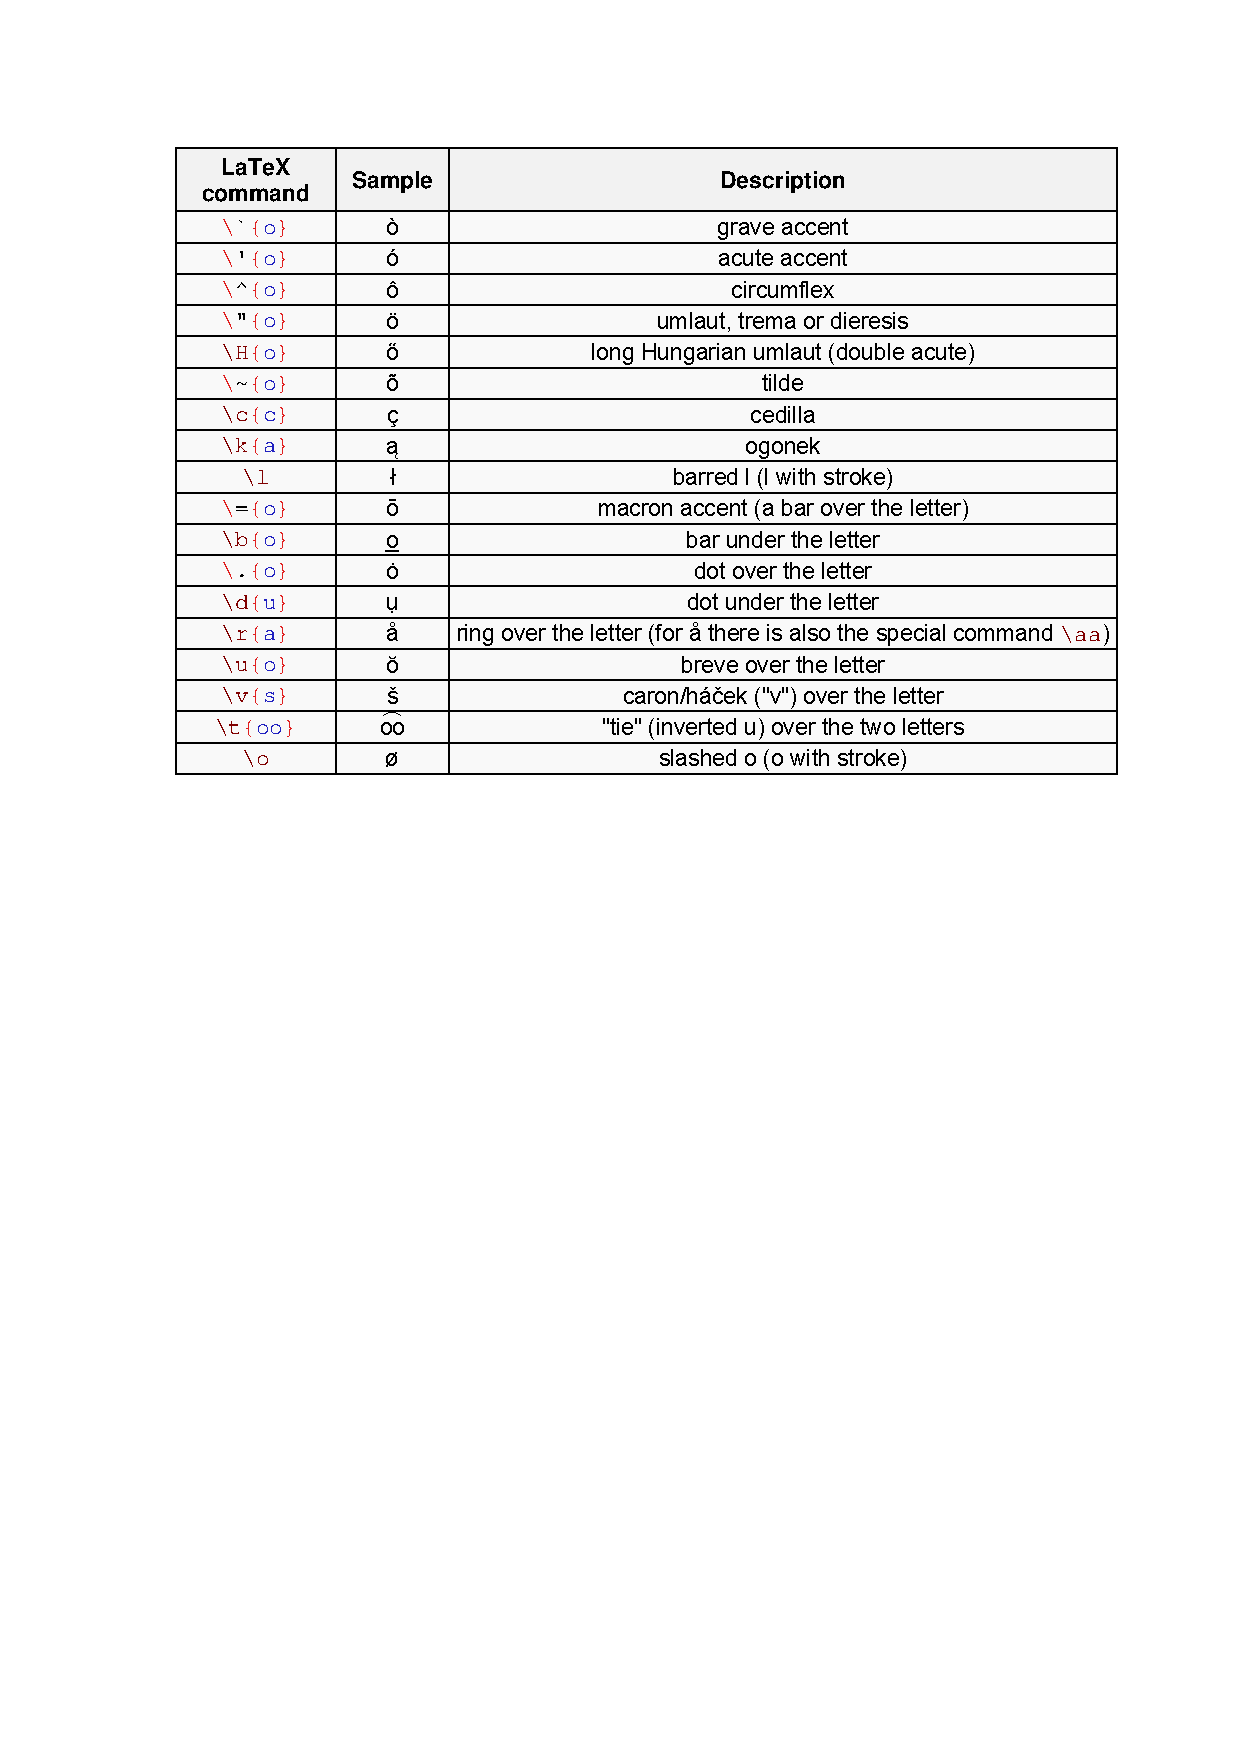
\includegraphics[width=0.8\textwidth]{./04-figuras/acentosLatex}
	\fonte{\href{http://en.wikibooks.org/wiki/LaTeX/Special_Characters}{http://en.wikibooks.org/wiki/LaTeX/Special\underline{ }Characters}}
	\label{fig:acentosLatex}
\end{figure}


Para a compilação de arquivos \TeX{} ou \LaTeX{} veja os comandos apresentados na \autoref{fig:comanCompilaTex}.


\begin{figure}[!htb]
	\centering
	\caption{Comandos para compilação de arquivos \TeX{} ou \LaTeX}
	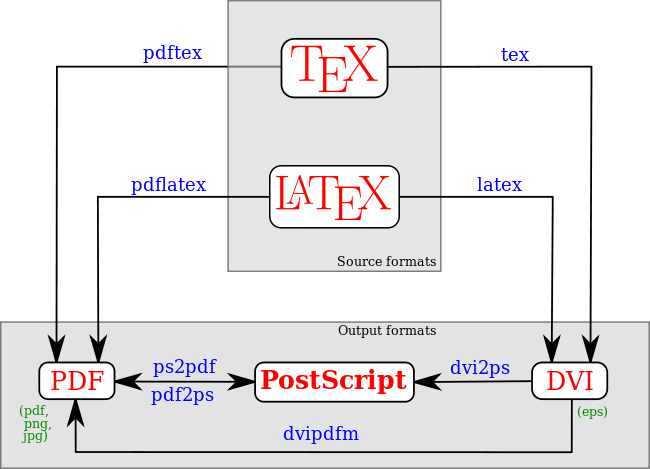
\includegraphics[width=0.8\textwidth]{./04-figuras/ComandosCompilacaoTex}
	\fonte{\href{http://en.wikibooks.org/wiki/LaTeX/Basics}{http://en.wikibooks.org/wiki/LaTeX/Basics}}
	\label{fig:comanCompilaTex}
\end{figure}


A compilação para gerar um arquivo no formato pdf, incluindo corretamente as referências bibliográficas, deve ser realizada em quatro passos:

\begin{compactitem}
	\item \textbf{pdflatex} \verb|meuTrabalhoAcademico.tex|    -> gera um pdf, porém sem as referências, apenas indicando-as
	\item \textbf{bibtex} \verb|meuTrabalhoAcademico.tex|	-> varre o arquivo myrefs.bib e busca pelas referências utilizadas
	\item \textbf{pdflatex} \verb|meuTrabalhoAcademico.tex|	-> insere as referências e chamadas nos locais apropriados
	\item \textbf{pdflatex} \verb|meuTrabalhoAcademico.tex|	-> faz a compilação final, verificando tudo
\end{compactitem}

Alternativamente, poderá ser utilizado o comando \verb|makefile|, disponível na mesma pasta onde está o arquivo principal \verb|meuTrabalhoAcademico.tex|, que faz exatamente o mesmo que os quatro comandos supramencionados. No entanto atente para o fato de que , se você alterar o nome do arquivo \verb|meuTrabalhoAcademico.tex|, deverá também editar o arquivo \verb|makefile| para alterá-lo do mesmo modo.

\section{Justificativa}
\label{sec:justificativa}

Blá blá blá .... 

			
% -----------------------------------------------------------------------------
%   Arquivo: ./02-elementos-textuais/metodologia.tex
% -----------------------------------------------------------------------------



\chapter{Metodologia}
\label{chap:metodologia}
O trabalho foi implementado na linguagem Python, versão 3.5 e interpretado no Linux Debian - Stretch 64 bits. 

Foram utilizados os seguintes parâmetros: 

\begin{table}[!htb]
	\centering
	\caption[Parametros utilizados]{Parametros utilizados.
	\label{tab:parametros}}
	\begin{tabular}{rrrrr}
		\toprule
			& Vetores & Tamanho de cada vetor & Valores aleatórios &  \\
		\midrule
			MaxMin1 & 500 & 10.000 & 0 a 1x10\textsuperscript{7} \\
			MaxMin2 & 500 & 10.000 & 0 a 1x10\textsuperscript{7} \\
		\bottomrule
	\end{tabular}
\end{table}



Para efeito ilustrativo, segue o código de implementação MaxMin1 em Python:\\

\begin{python}
def MaxMin1(A):
	Max = A[0]
	Min = A[0]
	j = int()
	
	for i in range(1, len(A)):
	
		j += 1 % Contador 
		if A[i] > Max:
		Max = A[i]
		
		j += 1 % Contador 
		if A[i] < Min:
		Min = A[i]
	
	return j 

\end{python}
		

\pagebreak

Já para o algoritmo Maxmin2, temos: \\

\begin{python}
def MaxMin2(A):
    Max = A[0]
    Min = A[0]
    j = int()

    for i in range(1, len(A)):

        j += 1 % Contador
        if A[i] > Max:
            Max = A[i]
            j += 1
        elif A[i] < Min:
            Min = A[i]

    return j % Retorna Contador
\end{python}



			
% -----------------------------------------------------------------------------
%   Arquivo: ./02-elementos-textuais/resultados.tex
% -----------------------------------------------------------------------------



\chapter{Análise e Discussão dos Resultados}

Como era de se esperar, o algoritmo MaxMin1 apresentou uma complexidade de 2(n-1), onde n é o tamanho do vetor, no caso, 10.000. Portanto, como ilustrado no gráfico abaixo, temos uma linha reta. Já para o algoritmo MaxMin2, percebemos uma performance melhor, uma vez que não temos a "comparação" de todos os elementos do vetor para encontrar o Maior e Menor valor. 

Segue a ilustração abaixo. 

\begin{figure}[!htb]
	\centering
	\caption{MaxMin1 x MaxMin2}
	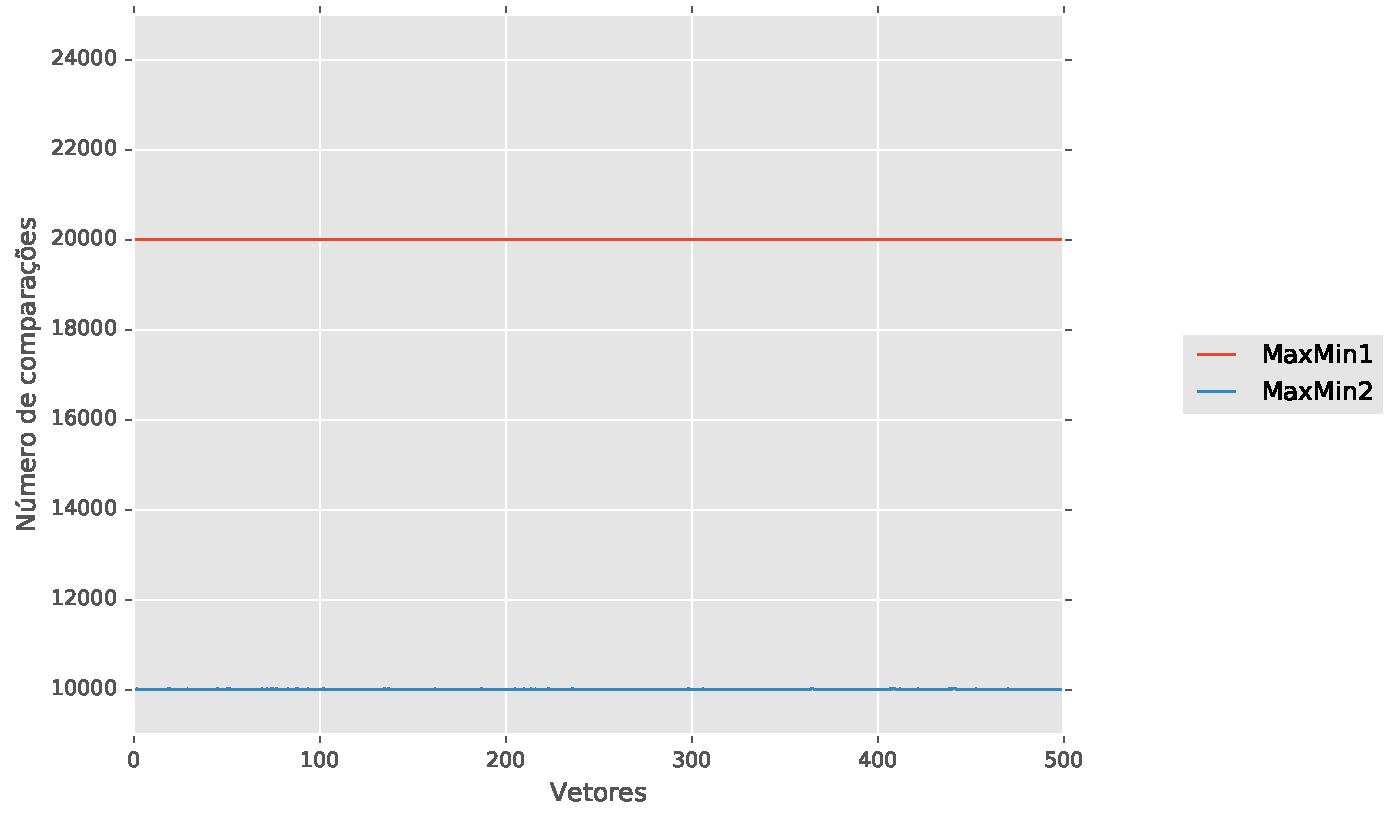
\includegraphics[width=0.8\textwidth]{./04-figuras/MaxMin1xMaxMin2.pdf}
	\fonte{Própria}
	\label{fig:maxmin1vsmaxmin2}
\end{figure}

\pagebreak
Apesar de não visivel (devido a escala do gráfico), o método MaxMin2 apresentou uma pequena variação de seus contadores. Esta pequena variação pode ser visualizada no gráfico abaixo onde a escala foi mudada. 


\begin{figure}[!htb]
	\centering
	\caption{MaxMin2}
	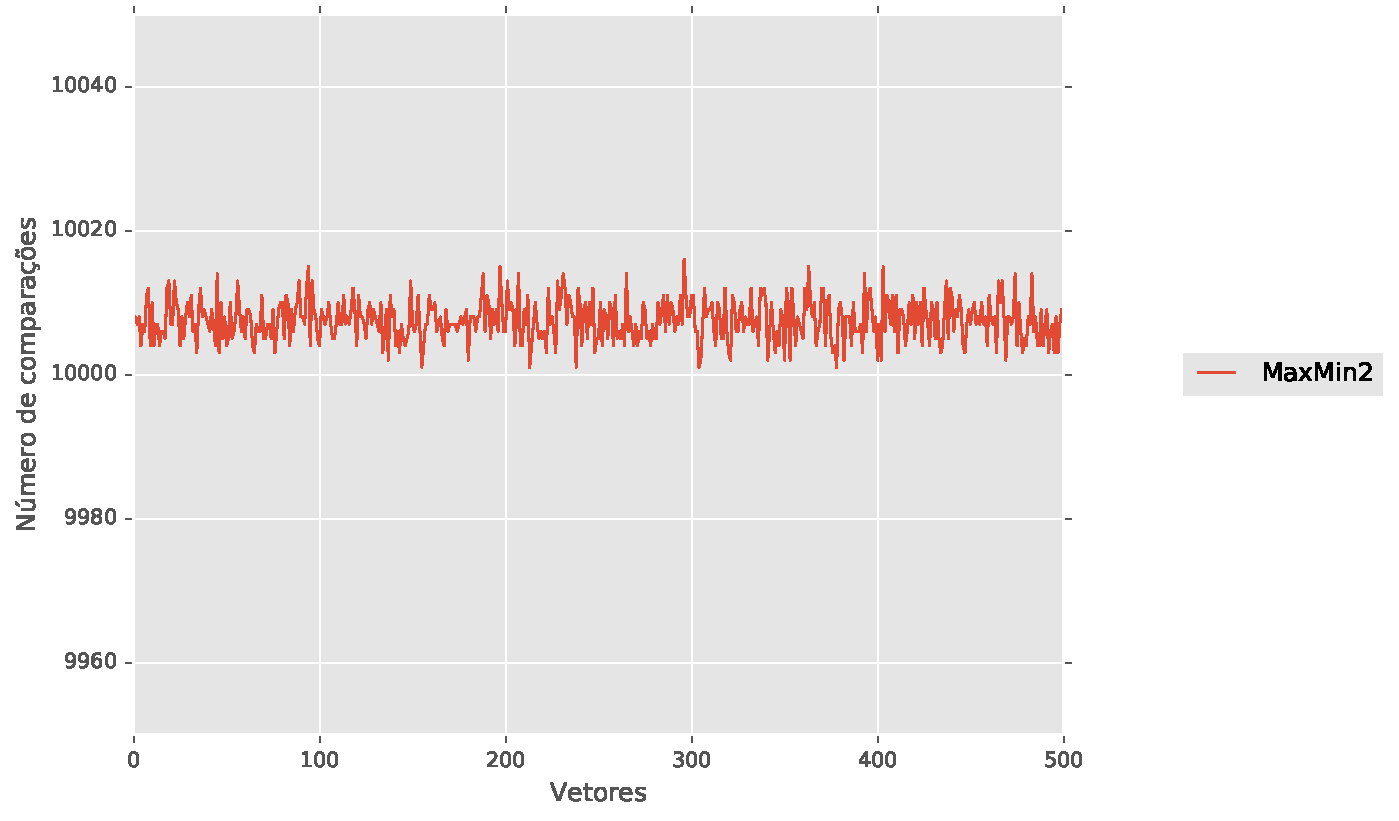
\includegraphics[width=0.8\textwidth]{./04-figuras/MaxMin2.pdf}
	\fonte{Própria}
	\label{fig:maxmin2}
\end{figure}



O valor médio encontrado pelo algoritmo MaxMin1 e MaxMin2 estão ilustrados na tabela a seguir: 

\begin{table}[!htb]
	\centering
	\caption[Médias encontradas]{Médias encontradas.
	\label{tab:medias}}
	\begin{tabular}{rrrrr}
		\toprule
			& Média &  \\
		\midrule
			MaxMin1 & 19998.00 \\
			MaxMin2 & 10007.74 \\
		\bottomrule
	\end{tabular}
\end{table}


		
%% -----------------------------------------------------------------------------
%   Arquivo: ./02-elementos-textuais/conclusao.tex
% -----------------------------------------------------------------------------



\chapter{Conclusão}
\label{chap:conclusao}

Procure fazer uma análise crítica de seu trabalho, destacando os principais resultados e as contribuições deste trabalho para a área de pesquisa.



\section{Trabalhos Futuros}
\label{sec:trabalhosFuturos}

Também deve indicar, se possível e/ou conveniente, como este trabalho pode ser estendido ou aprimorado.



\section{Considerações Finais}
\label{sec:consideracoesFinais}

As derradeiras palavras para encerramento do seu trabalho acadêmico.



% -----------------------------------------------------------------------------
%   OBS: a norma ABNT estabelece que em qualquer tipo de trabalho acadêmico monográfico
%   deve haver um capítulo de conclusão
% -----------------------------------------------------------------------------
				

%   Insere os elementos pós-textuais
\postextual
%% -----------------------------------------------------------------------------
%   Arquivo: ./03-elementos-pos-textuais/referencias.tex
% -----------------------------------------------------------------------------



% -----------------------------------------------------------------------------
%   Carrega o arquivo “myRefs.bib” e extrai automaticamente as referências citadas
% -----------------------------------------------------------------------------

\bibliography{./03-elementos-pos-textuais/myRefs}{}
\bibliographystyle{abntex2-alf}		% Define o estilo ABNT para formatar a lista de referências  


% -----------------------------------------------------------------------------
%   Este arquivo não necessita de ser editado.
% -----------------------------------------------------------------------------



\end{document}
